\section{Pendahuluan}
\subsection{Latar Belakang}

Pada modul pertama, praktikan mempelajari penggunaan osiloskop dan function generator.
Proses pengolahan sinyal digital, peralatan pengukuran dan pengujian sangatlah penting untuk memastikan bahwa sinyal yang diolah telah sesuai dengan spesifikasi yang diinginkan. Dalam konteks ini, osiloskop dan function generator merupakan peralatan yang sangat fundamental.
\\\\
Osiloskop merupakan alat ukur elektronik yang digunakan untuk melakukan visualisasi sinyal listrik dalam bentuk gelombang. Dengan osiloskop, kita dapat mengamati perubahan tegangan seiring waktu, yang sangat berguna untuk menganalisis karakteristik sinyal dalam rangkaian elektronik.
Osiloskop memungkinkan pengguna untuk: mengukur frekuensi dan periode sinyal, mengamati bentuk gelombang dan mendeteksi distorsi atau noise, mengukur tegangan puncak ke puncak (Vpp) dan tegangan rata-rata, dan menganalisis hubungan fasa antara dua sinyal.
\\\\
Function generator adalah alat yang digunakan untuk menghasilkan berbagai bentuk gelombang listrik, seperti gelombang sinus, persegi, segitiga, dan gigi gergaji. 
Function generator sangat berguna dalam pengujian dan pengembangan rangkaian elektronik karena memungkinkan pengguna untuk: menghasilkan sinyal dengan frekuensi dan amplitudo yang dapat diatur, menguji respons rangkaian terhadap berbagai bentuk gelombang, dan mensimulasikan kondisi operasi yang berbeda dalam rangkaian.
\\\\

\subsection{Maksud dan Tujuan}
Mengetahui dan memahami dasar penggunaan osiloskop dan function generator.

\subsection{Hasil yang diharapkan}
Dapat memahami dasar penggunaan osiloskop dan function generator.

%===========================================================%
\section{Tugas Pendahuluan}
\begin{enumerate}
\item Buatlah
\end{enumerate}

%===========================================================%
\section{Alat dan Bahan}
\begin{itemize}[label=$\bullet$, itemsep=-1pt, leftmargin=*]
	\item Buatlah
\end{itemize}

%===========================================================%
\section{Jangka Waktu Pelaksanaan}
Pemahaman dan konfigurasi 1 jam.

%===========================================================%

\section{Proses dan Tahapan Konfigurasi}
%======================PERCOBAAN 1==========================%
\subsection{Wireless Point to Point}
\begin{center}

	\textbf{Konfigurasi Router 1}
	\begin{enumerate}
		\item Buka aplikasi WinBox pada PC 1 dan lakukan koneksi ke Router 1.\\Neighbors > Refresh > Double click Router yang terdeteksi > Connect
			\begin{figure}[H]
				\centering
				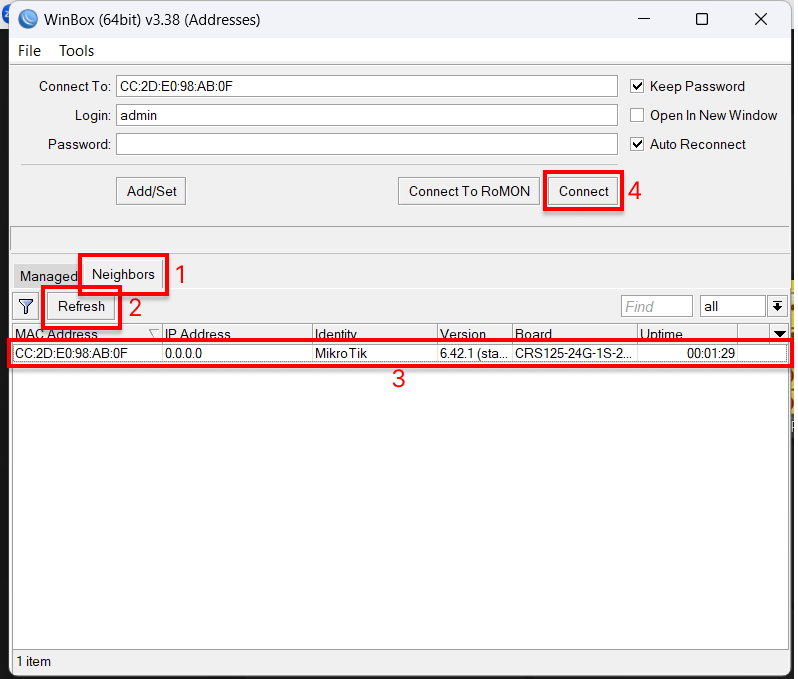
\includegraphics[width=0.8\linewidth]{P1/img/per1/pc1/Step 1.png}
				\caption{Step 1}
				\label{fig:Step 1(Per.1 PC1)}
			\end{figure}
	\end{enumerate}

	\textbf{Konfigurasi Router 2}
	\begin{enumerate}
		\item Buka WinBox dan lakukan koneksi ke Router
			\begin{figure}[H]
				\centering
				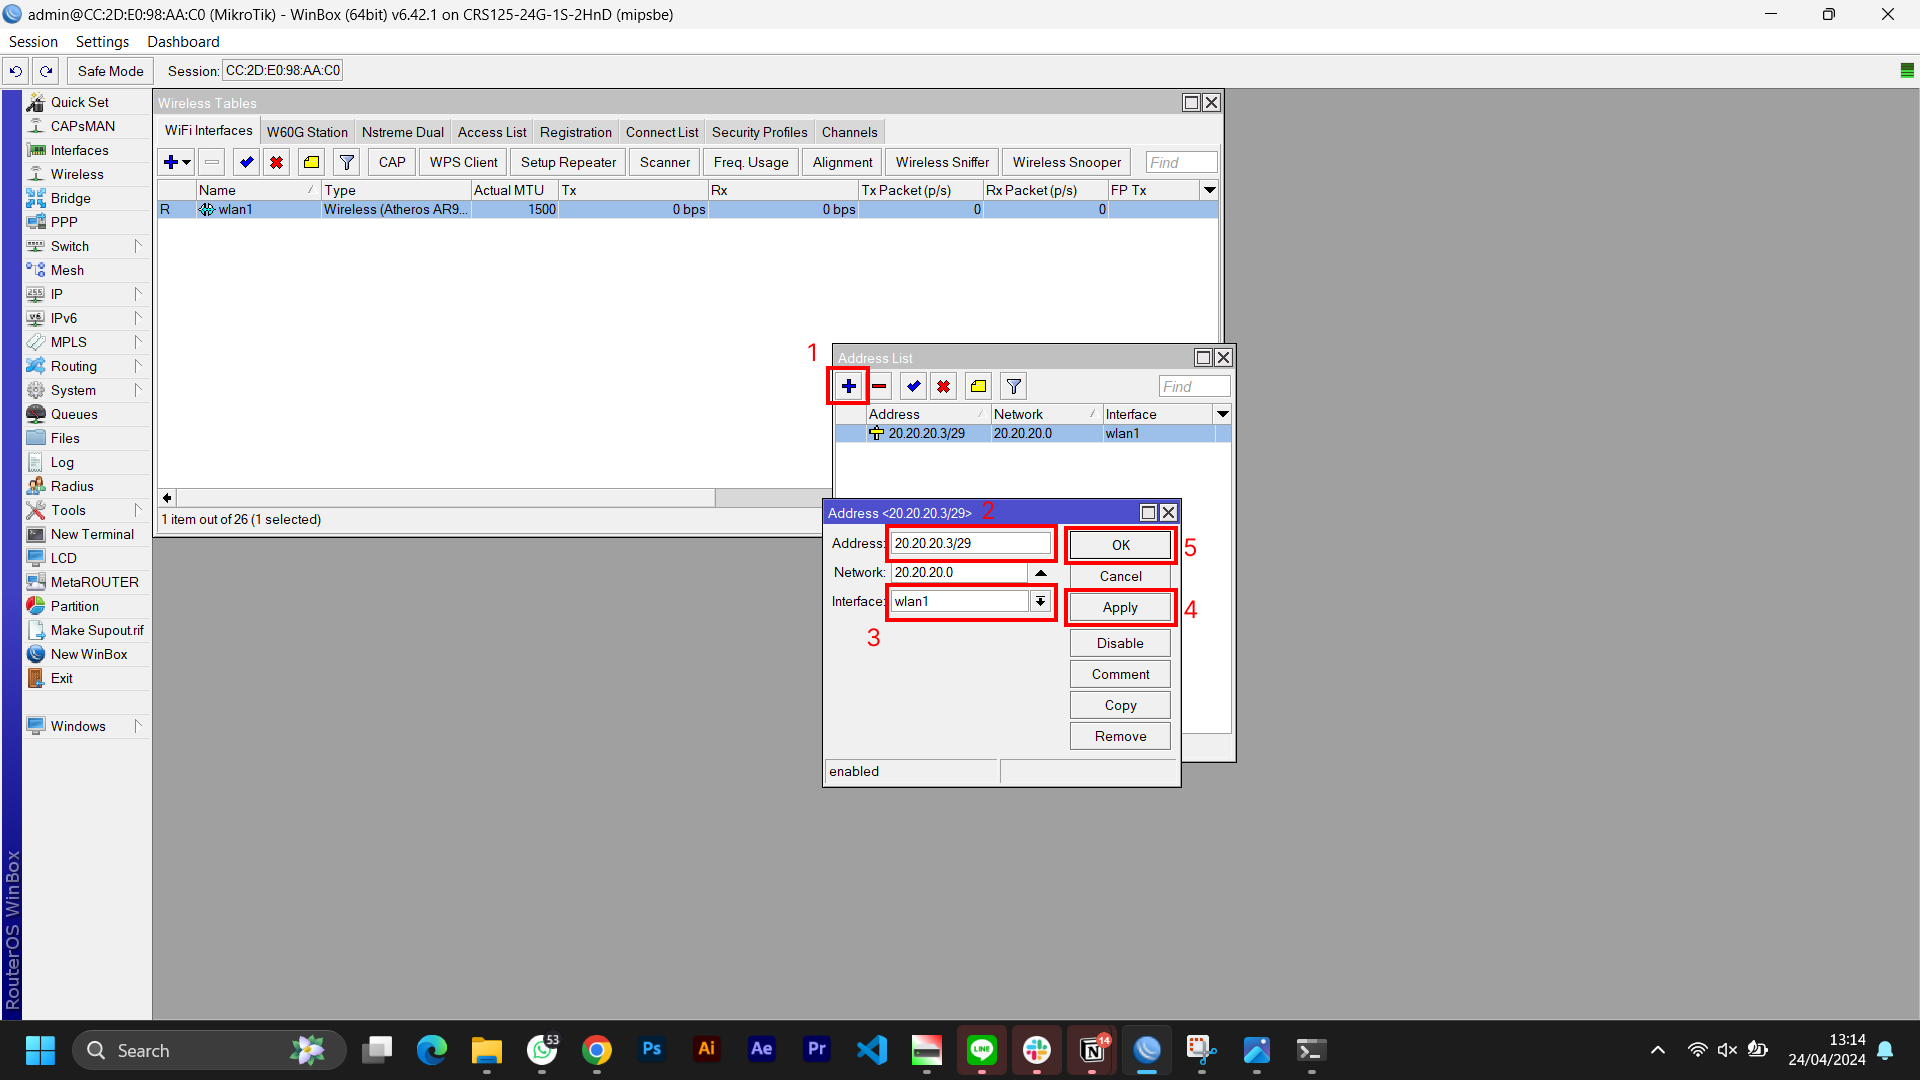
\includegraphics[width=0.9\linewidth]{P1/img/per1/pc2/Step 2.png}
				\caption{Step 2}
				\label{fig:Step 2(Per.1 PC2)}
			\end{figure}
	\end{enumerate}

	\textbf{Pengujian konfigurasi}
	\begin{enumerate}
	\item Lakukan test ping dari Router 1 ke Router 2
	\begin{figure}[H]
		\centering
		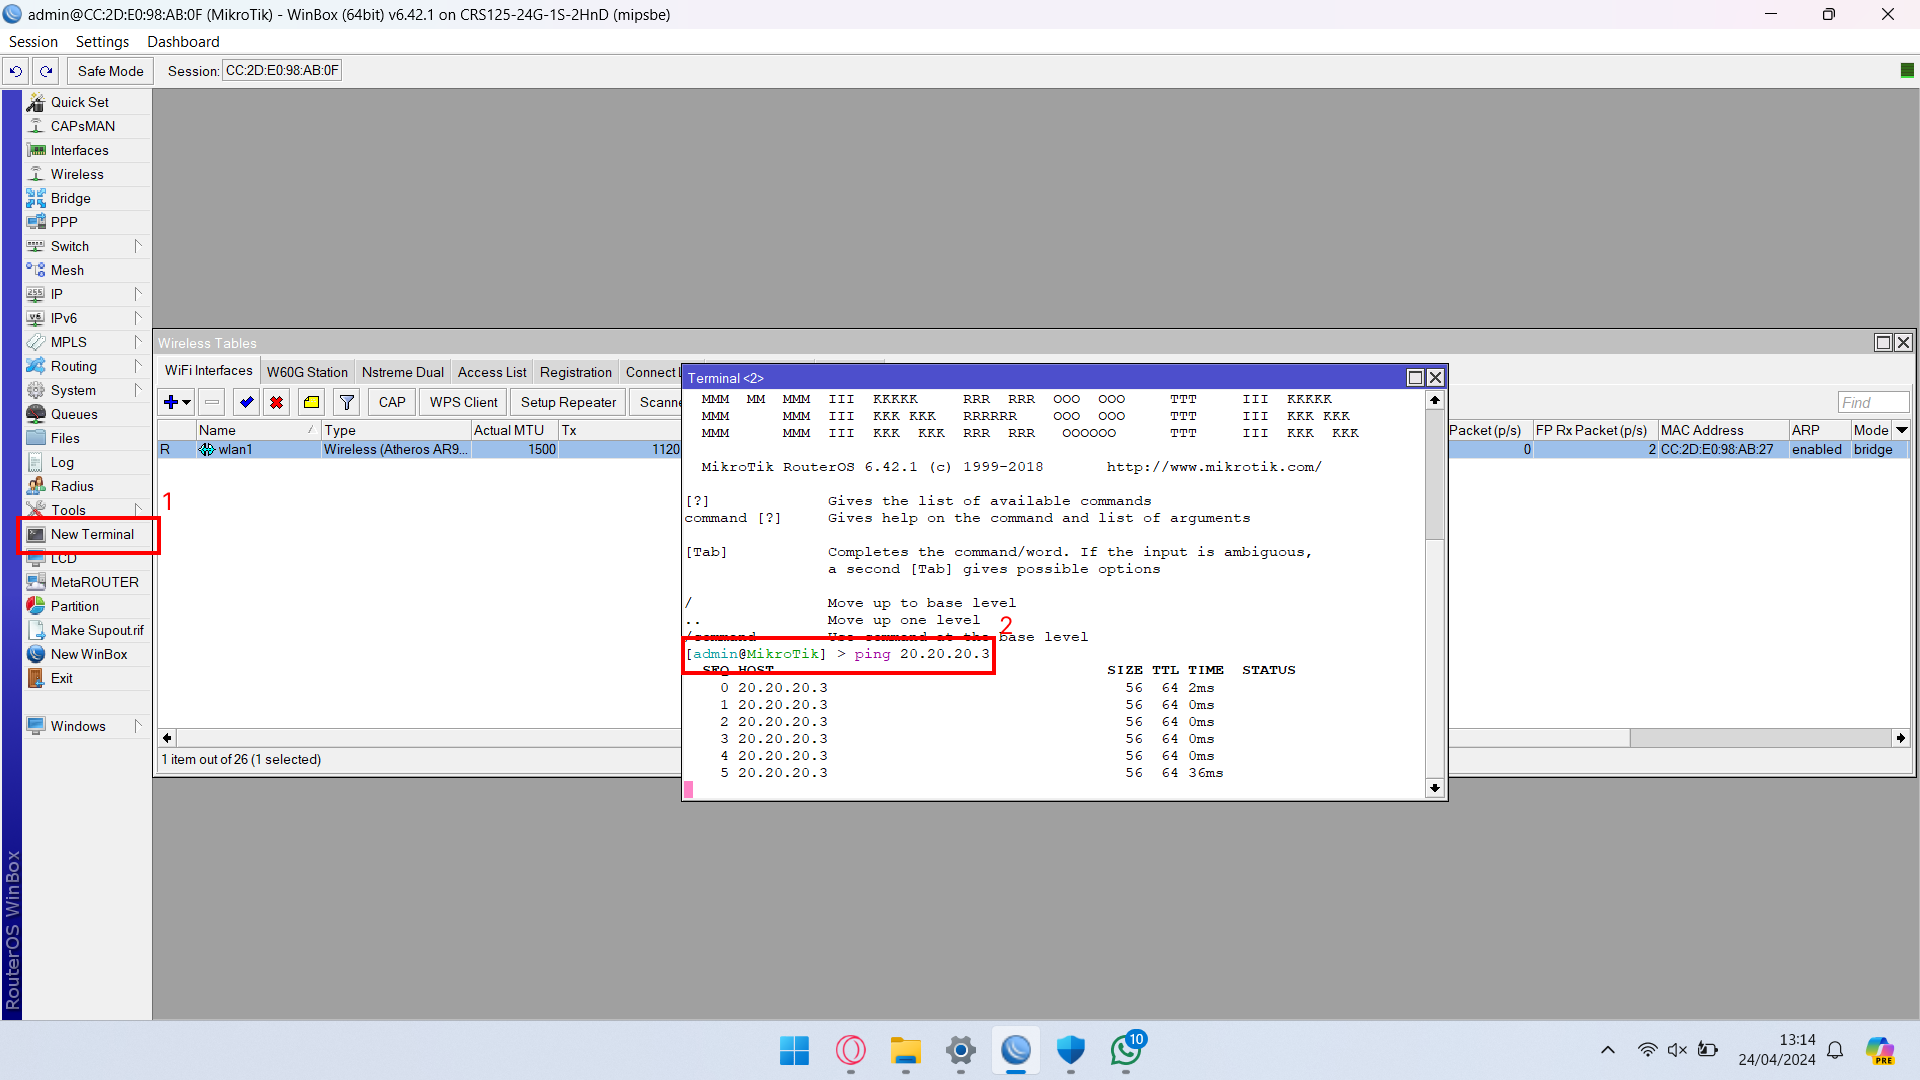
\includegraphics[width=0.9\linewidth]{P1/img/per1/pc1/Step 4.png}
		\caption{Step 1}
		\label{fig:Ping Step 1(Per.1 PC1)}
	\end{figure}
	\end{enumerate}
\end{center}

%======================PERCOBAAN 2==========================%
\subsection{Wireless Point to Multipoint}
\begin{center}

	\textbf{Konfigurasi Router 1}
	\begin{enumerate}
		\item Berikan IP address sesuai dengan cara pengaturan IP address yang benar. Berikan IP address yang berbeda dengan contoh di modul.
		      \begin{figure}[H]
			      \centering
			      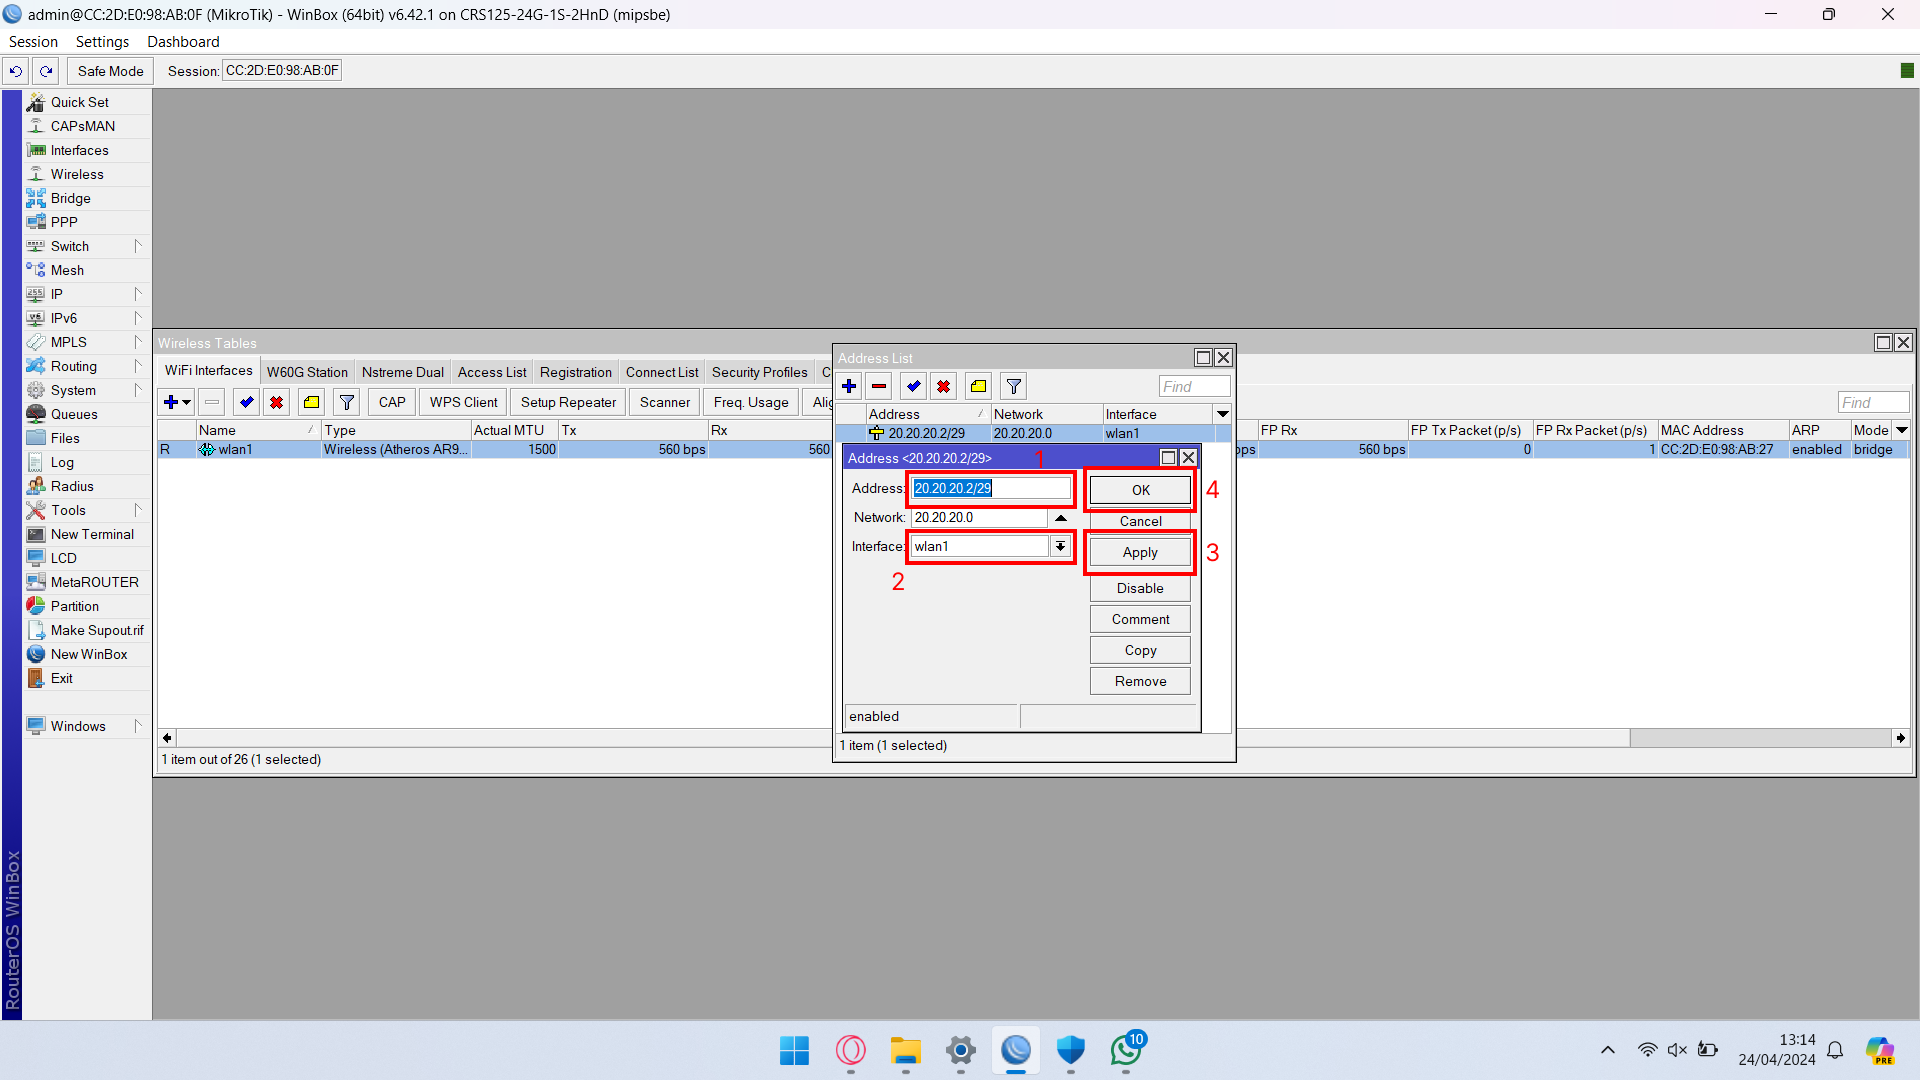
\includegraphics[width=0.9\linewidth]{P1/img/per1/pc1/Step 2.2.png}
			      \caption{Step 1}
			      \label{fig:Step 1(Per.2 PC1)}
		      \end{figure}
	\end{enumerate}

	\textbf{Konfigurasi Router 2}
	\begin{enumerate}
		\item Berikan IP address pada interface wlan 1 yang dapat dibuat pada tab IP > Addresses. Berikan IP address sesuai dengan cara pengaturan IP address yang benar. Berikan IP address yang berbeda dengan contoh di modul.
		      \begin{figure}[H]
			      \centering
			      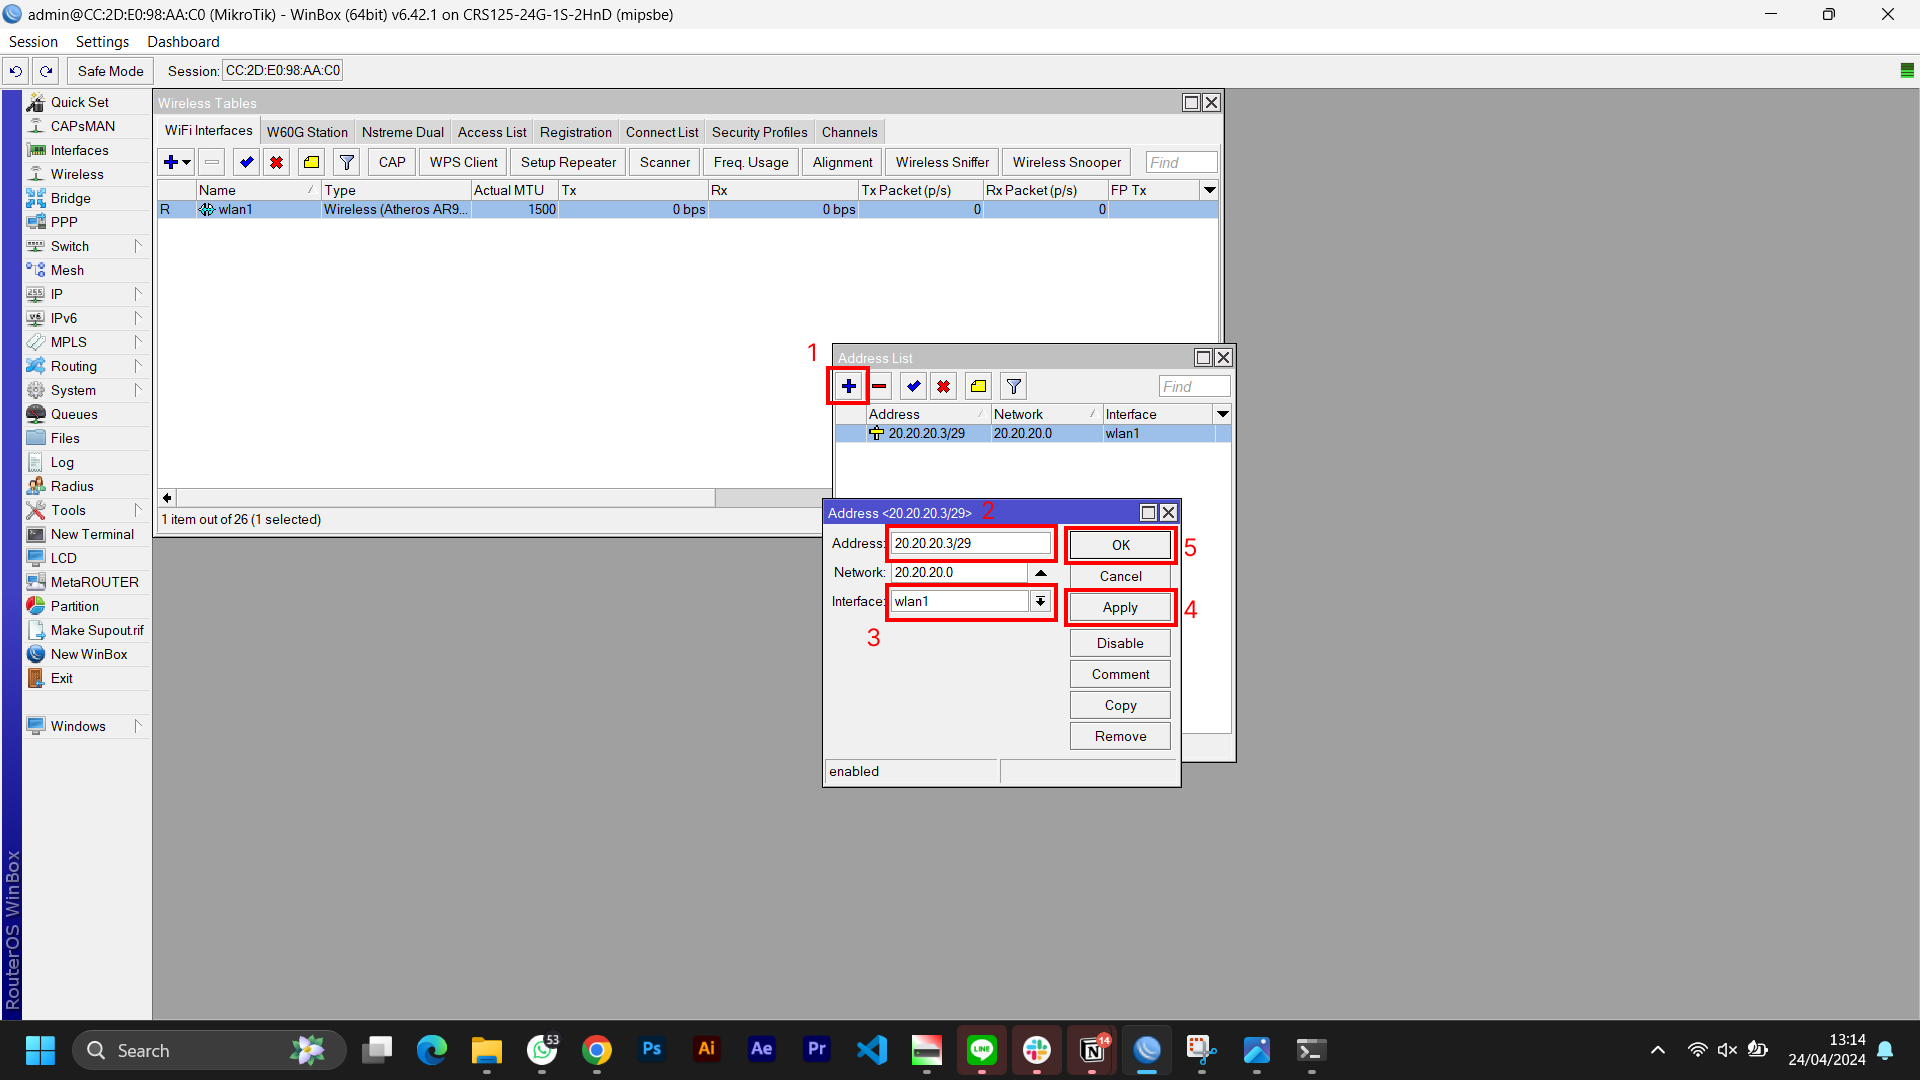
\includegraphics[width=0.9\linewidth]{P1/img/per1/pc2/Step 2.png}
			      \caption{Step 1}
			      \label{fig:Step 1(Per.2 PC2)}
		      \end{figure}
	\end{enumerate}

	\textbf{Pengujian konfigurasi}
	\begin{enumerate}
		\item Lakukan test ping dari Router 1 ke Router 2
		      \begin{figure}[H]
			      \centering
			      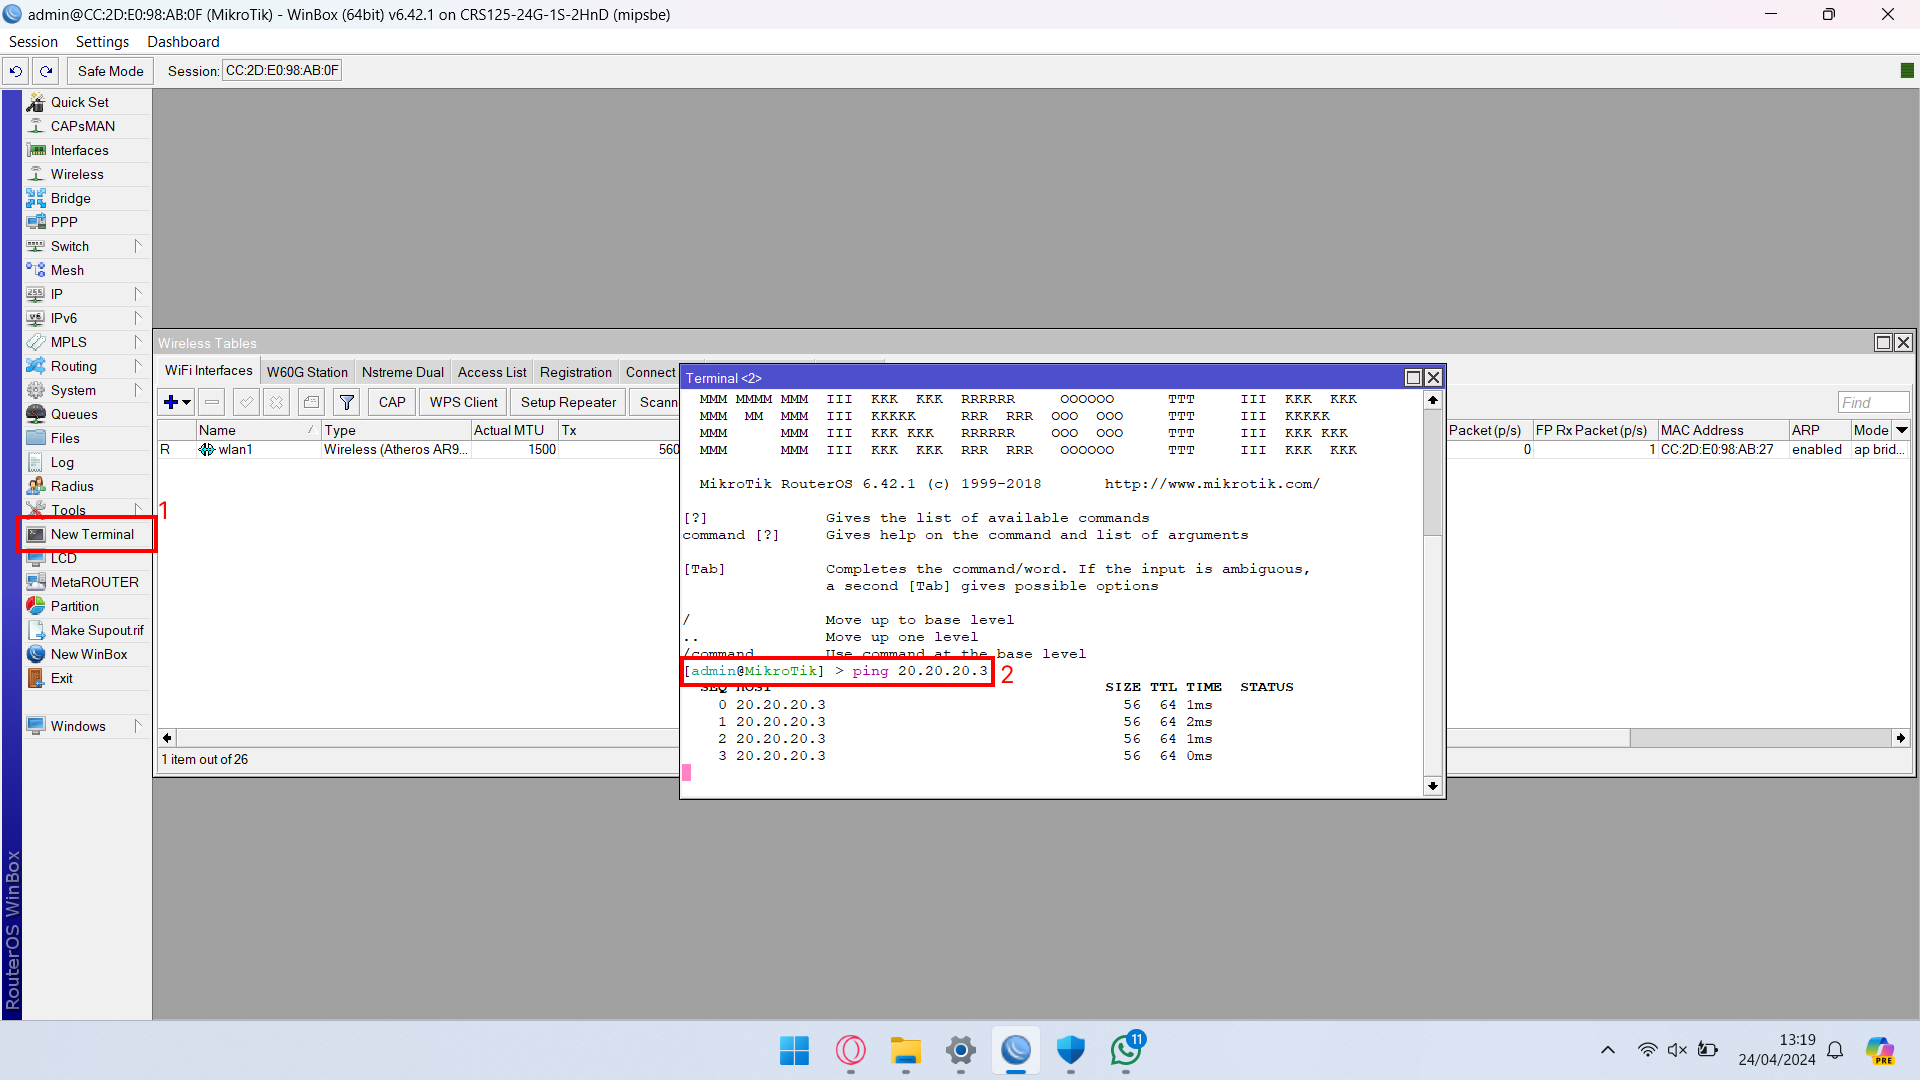
\includegraphics[width=0.9\linewidth]{P1/img/per2/pc1/Step 4.png}
			      \caption{Step 1}
			      \label{fig:Ping Step 1(Per.2 PC1)}
		      \end{figure}
	\end{enumerate}

\end{center}

%======================PERCOBAAN 3==========================%
\subsection{Wireless Bridge}
\begin{center}

	\textbf{Konfigurasi Router 1}
	\begin{enumerate}
		\item Buka WinBox dan lakukan koneksi ke Router
		      \begin{figure}[H]
			      \centering
			      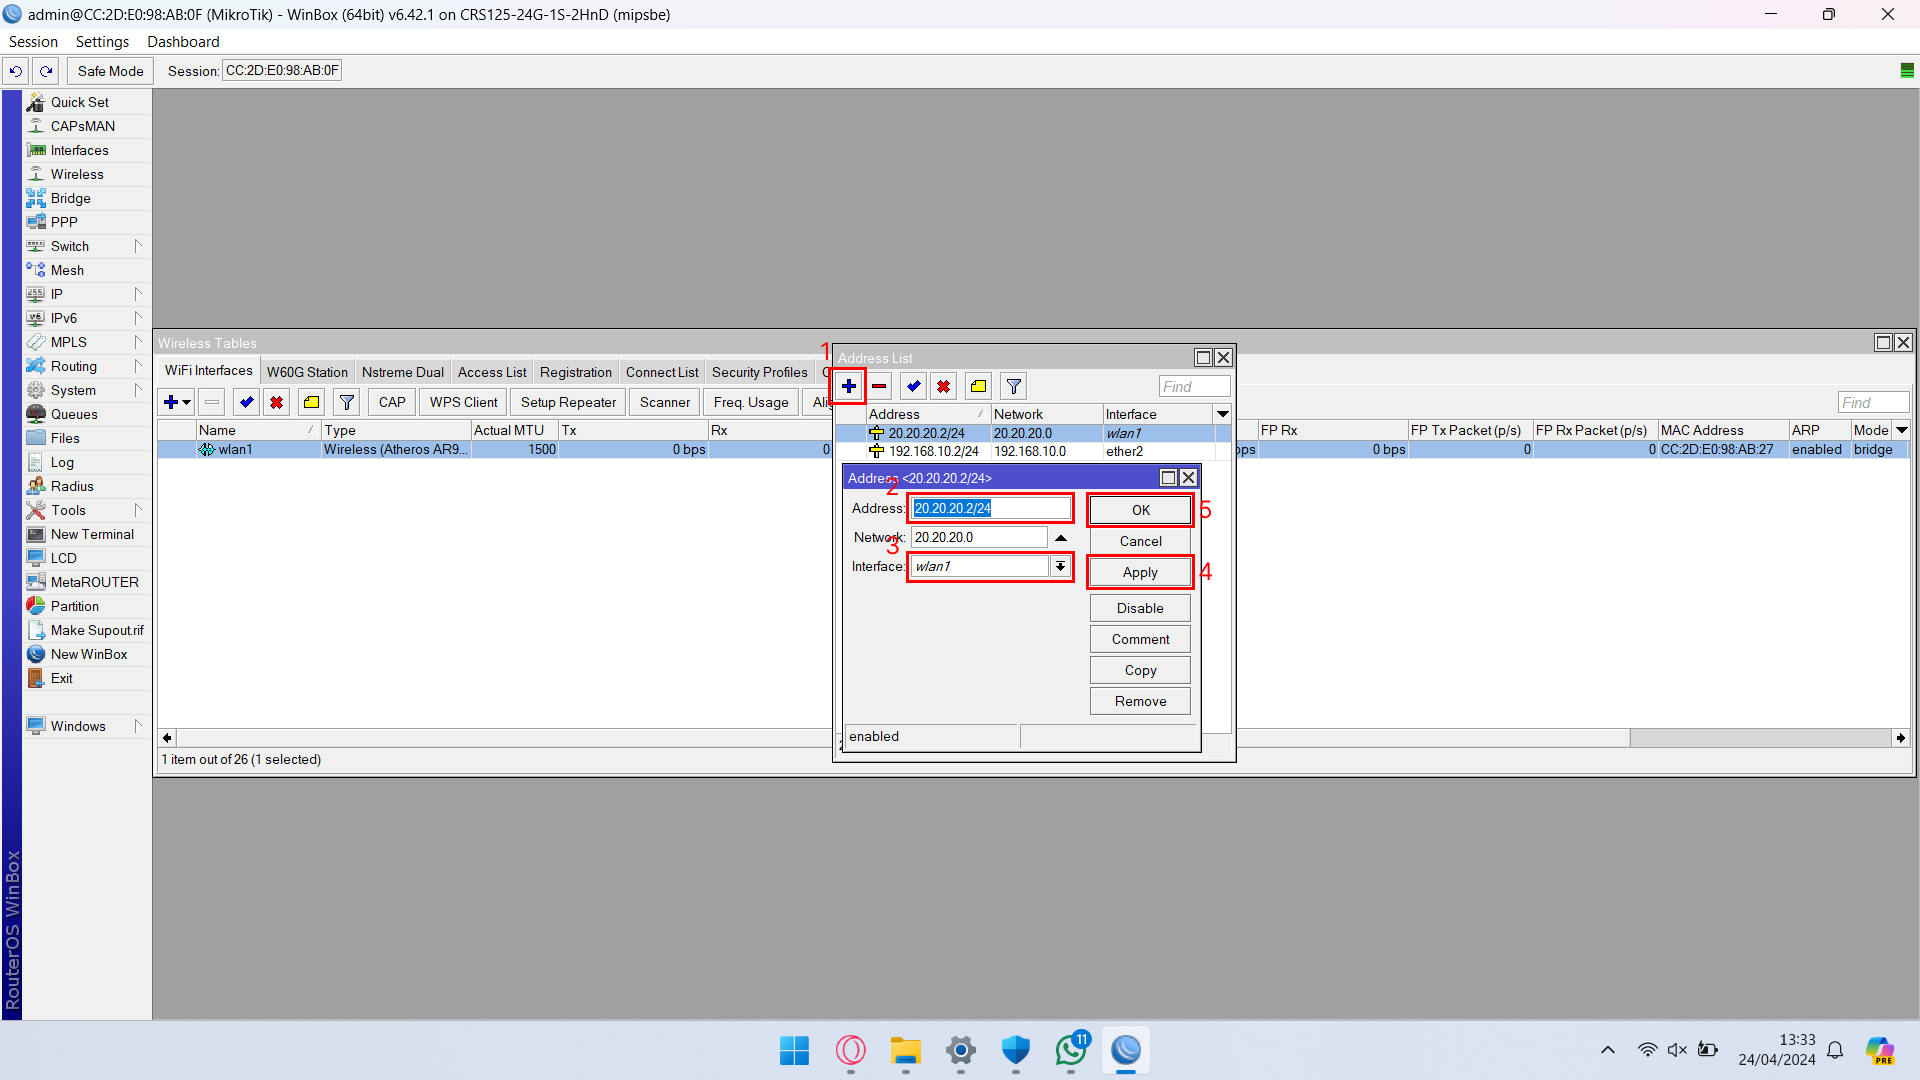
\includegraphics[width=0.9\linewidth]{P1/img/per3/pc1/Step 2.png}
			      \caption{Step 2}
			      \label{fig:Step 2(Per.3 PC1)}
		      \end{figure}
	\end{enumerate}

	\textbf{Konfigurasi Router 2}
	\begin{enumerate}
		\item Berikan IP address pada interface wlan1 dan ethernet 2 yang dapat dibuat pada tab IP > Addresses. Berikan IP address sesuai dengan cara pengaturan IP address yang benar. Berikan IP address yang berbeda dengan contoh di modul.
		      \begin{figure}[H]
			      \centering
			      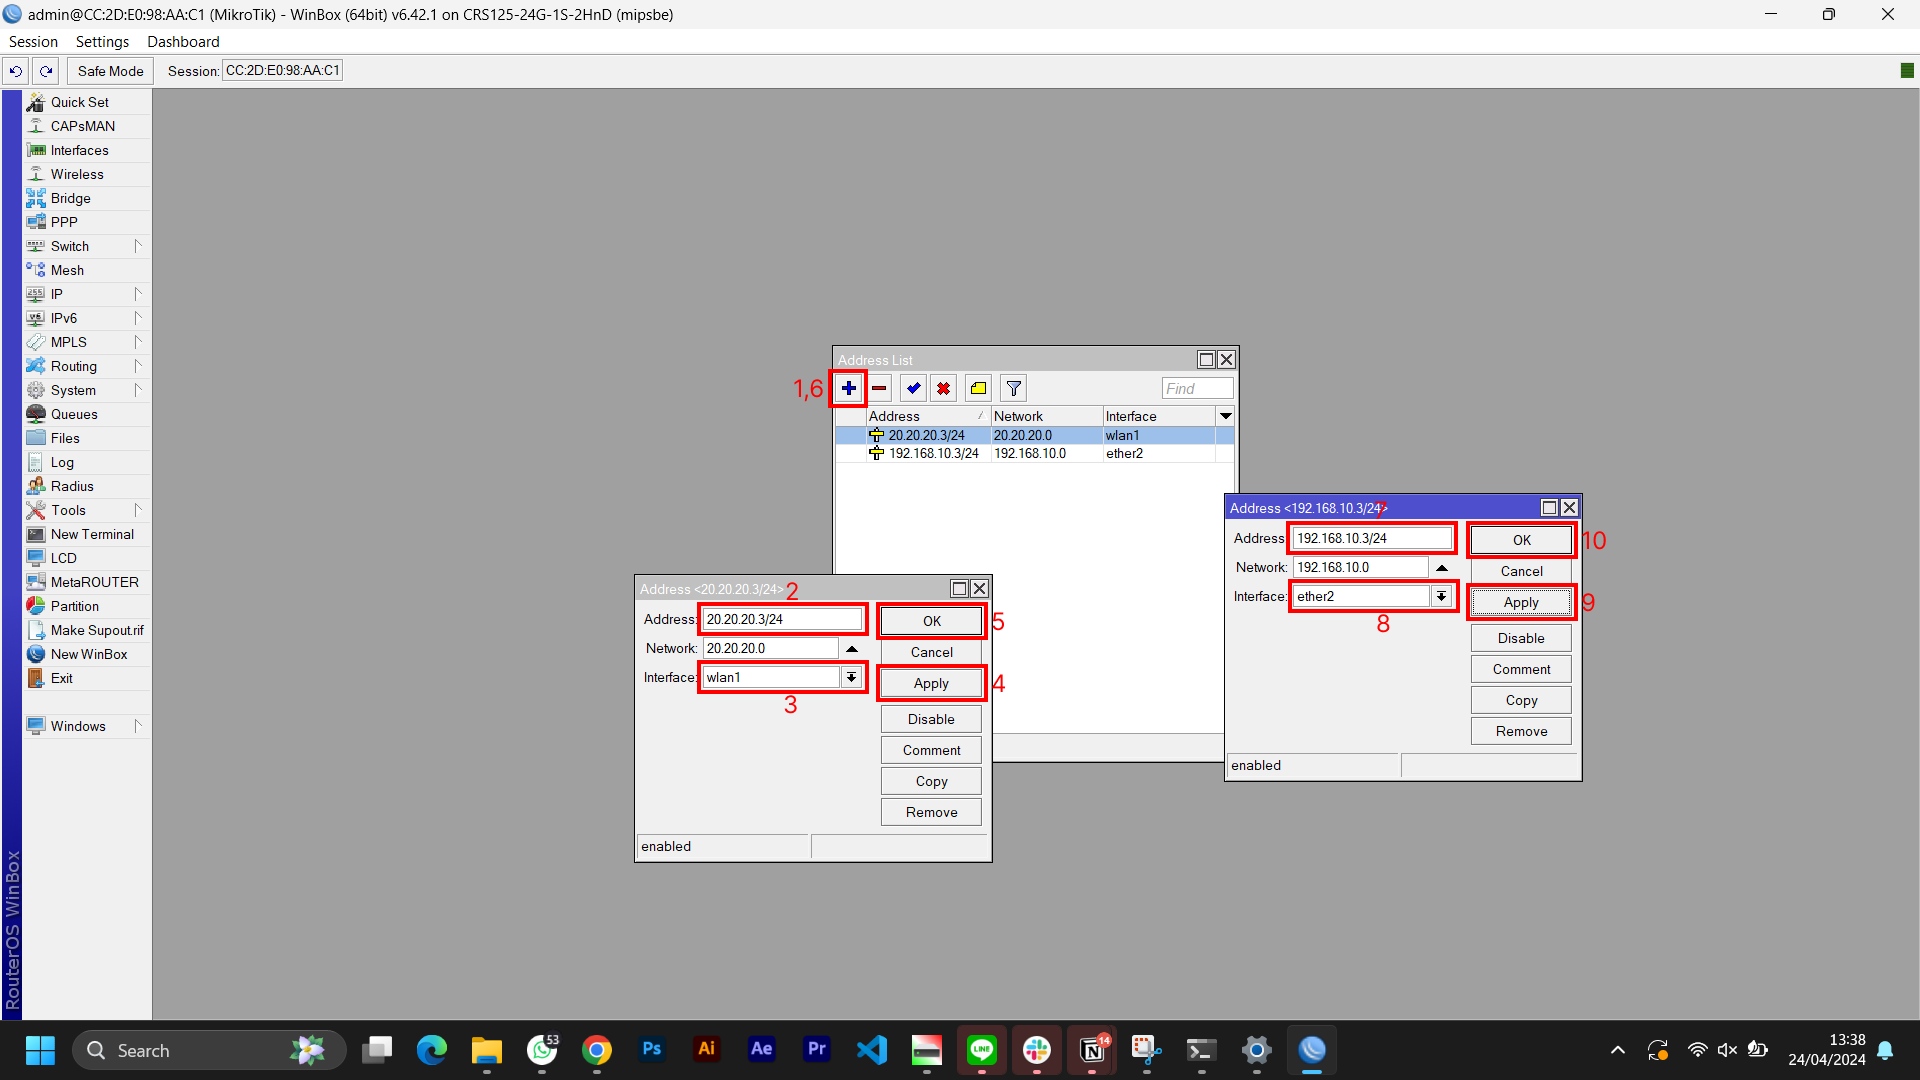
\includegraphics[width=0.9\linewidth]{P1/img/per3/pc2/Step 2.png}
			      \caption{Step 2}
			      \label{fig:Step 2(Per.3 PC2)}
		      \end{figure}
	\end{enumerate}

	\textbf{Pengujian konfigurasi}
	\begin{enumerate}
		\item Lakukan test ping dari PC 1 ke PC 2
		      \begin{figure}[H]
			      \centering
			      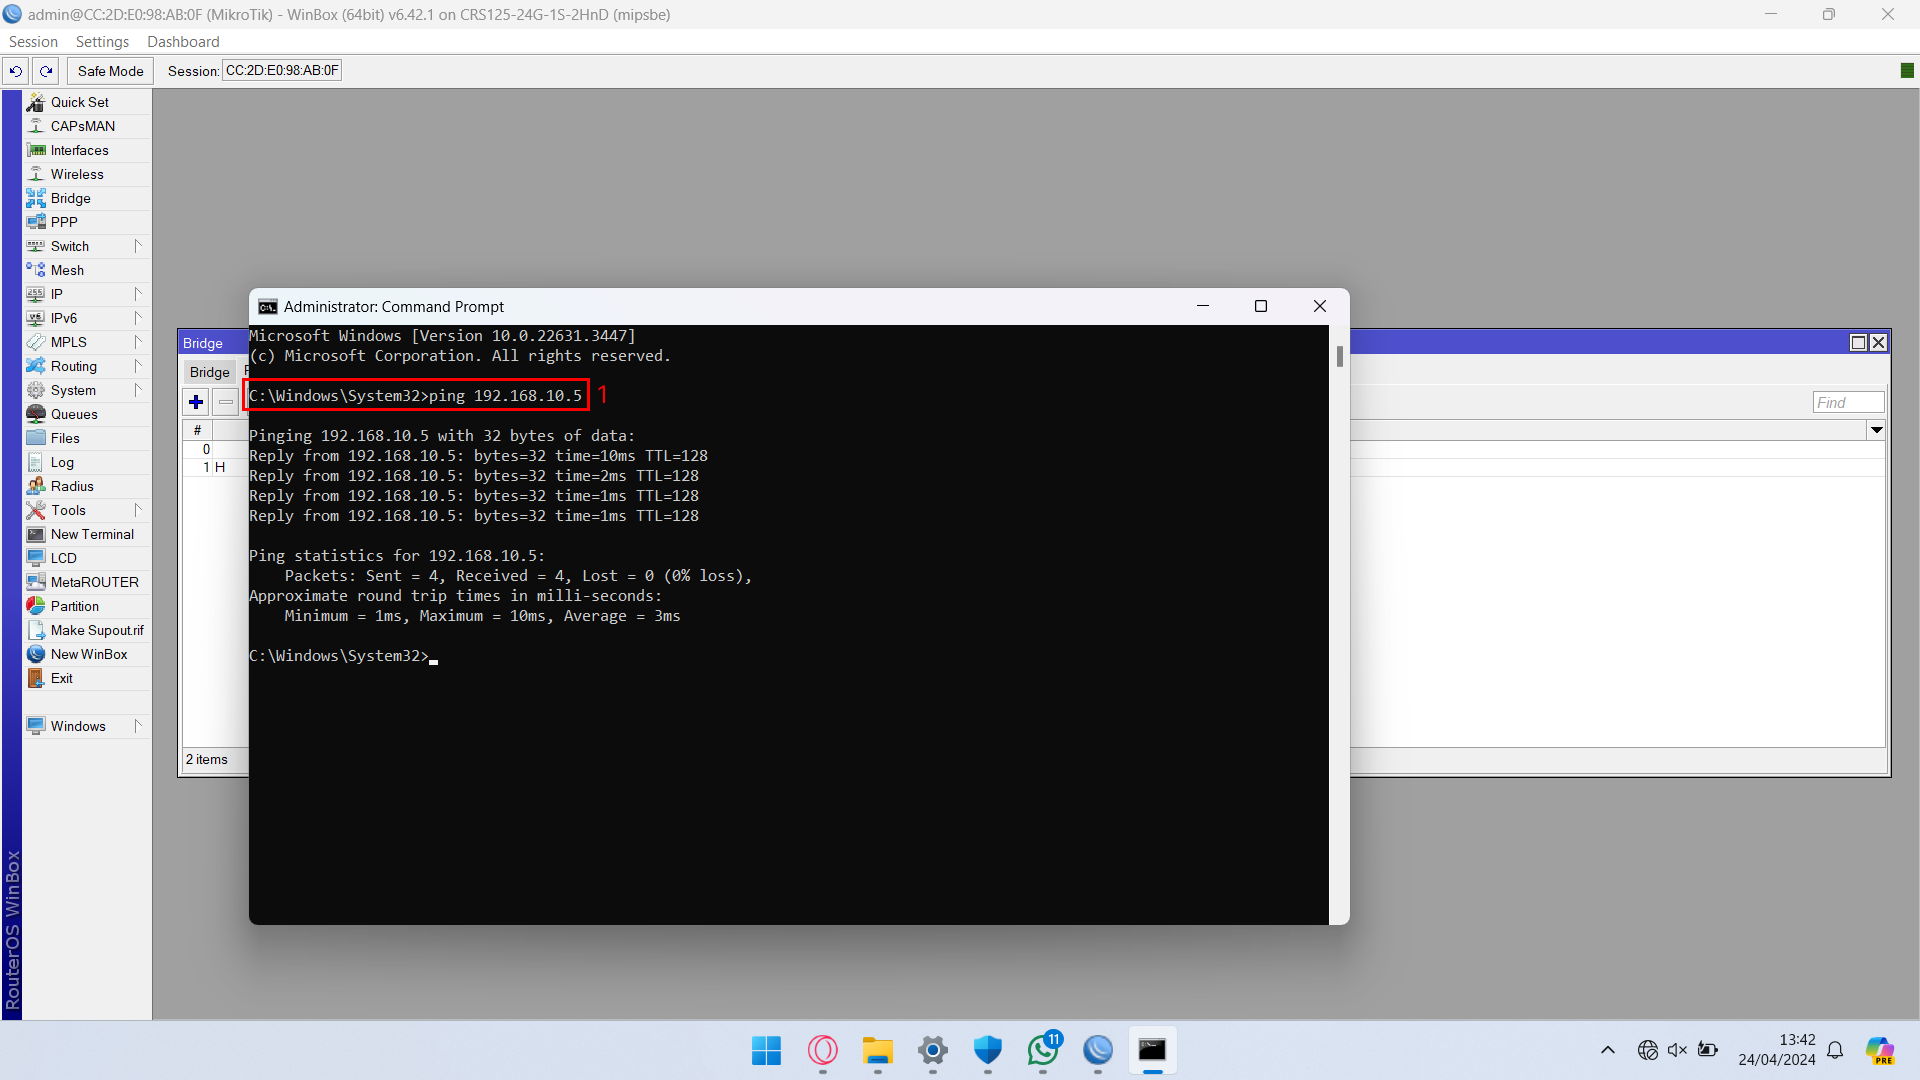
\includegraphics[width=0.9\linewidth]{P1/img/per3/pc1/Step 7.png}
			      \caption{Step 7}
			      \label{fig:Step 7(Per.3 PC1)}
		      \end{figure}
	\end{enumerate}

\end{center}

%===========================================================%
\section{Hasil yang didapat}
Memahami dan mengkonfigurasi koneksi Point to Point, Point to Multipoint dan Wireless
Bridging dengan tepat.

%===========================================================%
\section{Temuan Permasalahan}
Firewall hidup pada Laptop dapat mempengaruhi koneksi wireless tidak terhubung, kalian
bisa menonaktifkan firewall di laptop kalian, tetapi hal ini tidak terjadi di semua perangkat.

%===========================================================%
\section{Kesimpulan}
Dengan memahami dan mengkonfigurasi 3 jenis koneksi pada wireless, kita dapat
mengimplementasikan koneksi wireless dengan tepat sesuai kebutuhan dan kondisi tertentu.
